% !TeX root = main.tex
\documentclass[11pt]{article}

\usepackage{arxiv}

\usepackage[utf8]{inputenc}
\usepackage[T1]{fontenc}
\usepackage{hyperref}
\usepackage{url}
\usepackage{booktabs}
\usepackage{amsmath}
\usepackage{amsfonts}
\usepackage{graphicx}
\usepackage{microtype}
\usepackage{natbib}
\usepackage{doi}
\usepackage{xcolor}
\usepackage{cleveref}

\graphicspath{{data/figures/}}

\title{PrefBench: A Benchmark Prototype for Personalized Pricing Agents under Hidden Buyer Preferences}

\author{
  Yingjie Lei\\
  University of Aberdeen\\
  \texttt{u19yl22@abdn.ac.uk}
}

\renewcommand{\shorttitle}{PrefBench}

\hypersetup{
  pdftitle={PrefBench: A Benchmark Prototype for Personalized Pricing Agents under Hidden Buyer Preferences},
  pdfsubject={personalized pricing, negotiation, benchmark, hidden preferences},
  pdfauthor={Yingjie Lei},
  pdfkeywords={personalized pricing, negotiation, benchmark, hidden buyer preferences, reinforcement learning}
}

\begin{document}
\maketitle

\begin{abstract}
Personalized pricing is difficult when buyers differ in their willingness to pay, feature preferences, and negotiation behavior, while the seller observes only partial information at the start of an interaction. This report presents PrefBench, a simulator-based benchmark prototype for studying personalized pricing agents under hidden buyer preferences. PrefBench instantiates the setting in configurable vehicle-feature pricing, but treats the domain as a controlled substrate for a broader problem: sequential pricing and negotiation under incomplete buyer information. The benchmark combines a structured product catalog, a semi-synthetic persona bank with observable and latent buyer attributes, a multi-round negotiation environment, and a shared evaluation protocol for comparing pricing policies. We report checkpoint-free heuristic baselines under the same test protocol and use them as anchors for a planned zero-shot LLM evaluation path. The current release is intended as a working benchmark prototype rather than a comprehensive benchmark. We therefore document its simulator assumptions, limitations, and extension path toward LLM agents, belief probing, robustness evaluation, and human reference studies.

\end{abstract}

\keywords{Personalized pricing \and Negotiation agents \and Benchmark prototype \and Hidden buyer preferences \and Simulator-based evaluation}

\section{Introduction}
\label{sec:introduction}

Personalized pricing is a common decision problem in settings where a seller offers configurable products to buyers with heterogeneous preferences. A buyer may value the same bundle differently depending on budget, use case, feature priorities, and willingness to negotiate. This makes pricing more than a one-shot demand-estimation problem: the seller must decide how aggressively to price while observing only partial evidence about the buyer's latent preferences.

This report studies personalized pricing through a controlled benchmark prototype. The concrete substrate is customized vehicle-feature pricing, where a seller negotiates over a fixed feature bundle. The domain is useful because it combines feature-level value, implementation cost, buyer heterogeneity, and multi-round negotiation. However, the intended benchmark question is broader than vehicle customization: how should pricing agents be evaluated when buyer preferences are hidden and can only be inferred through interaction?

PrefBench is positioned between dynamic pricing, negotiation environments, and agent benchmark design. It provides a simulator-based benchmark for seller-side pricing decisions in a structured negotiation setting, with fixed assets, fixed persona splits, and shared evaluation metrics.

The contribution of this report is intentionally scoped. We release and document a working benchmark prototype rather than claiming a complete benchmark suite. The prototype includes a product catalog, persona generation pipeline, frozen persona bank, multi-round negotiation environment, and baseline evaluation protocol. We also outline how the benchmark can be extended to LLM agents, belief probing, robustness evaluation, and human reference studies.

The main contributions are:
\begin{itemize}
  \item We define a simulator-based benchmark prototype for personalized pricing and negotiation under hidden buyer preferences.
  \item We implement a reproducible environment with a structured catalog, semi-synthetic buyer personas, fixed data splits, and shared episode-level metrics.
  \item We report checkpoint-free heuristic baseline results under a common evaluation protocol and define the next LLM-facing evaluation path.
  \item We document the limitations of the current prototype and identify concrete future extensions for LLM-facing evaluation, belief probing, robustness testing, and human reference comparison.
\end{itemize}

\section{Related Work}
\label{sec:related_work}

\paragraph{Dynamic and personalized pricing.}
Dynamic pricing has been studied through contextual pricing, demand estimation, and learning-based price adjustment \citep{choi2023SemiParametricContextualPricing,liu2021DynamicPricingEcommerce,pandey2020DeepReinforcementLearning}. Personalized pricing additionally raises questions about consumer heterogeneity, fairness perception, and how individual or segment-level information should be used \citep{biggs2021ModelDistillationRevenue,dube2017PersonalizedPricingConsumer,priester2020SpecialPriceJust}. PrefBench differs from this line by focusing on a controlled benchmark setting with latent buyer traits and multi-round negotiation, rather than on a deployable pricing model or a single empirical market.

\paragraph{Negotiation agents and environments.}
Automated negotiation has a long history in multi-agent systems, including shared platforms and competitions such as ANAC and Genius \citep{baarslag2012FirstAutomatedNegotiating,lin2014GeniusIntegratedEnvironment}. NegMAS provides another research-oriented framework for constructing negotiation simulations \citep{mohammad2021NegMASPlatformAutomated}. More recent work has also evaluated bargaining abilities in language models \citep{xia2024MeasuringBargainingAbilities,chan2024NegotiationToMBenchmarkStresstesting}. PrefBench is related to these efforts, but its task is seller-side personalized pricing over configurable product features, with explicit profit, deal, and walkaway metrics.

\paragraph{Simulation benchmarks and research environments.}
Standardized simulator environments are useful when real interaction data are costly, sensitive, or difficult to control. Synthetic or simulator-based benchmarks are used in retail and pricing simulation settings \citep{xia2023RetailSynthSyntheticData,villarrubia-martin2025DynamicPricingHighSpeed}. PrefBench follows this simulator-based tradition while making its assumptions explicit: observable buyer profiles and hidden preference variables are generated under a controlled semi-synthetic process, and the current release is positioned as a benchmark prototype rather than a complete real-market substitute.

\section{Benchmark Design}
\label{sec:benchmark}

PrefBench evaluates a seller-facing pricing agent interacting with a buyer over a configurable product bundle. At each episode, the buyer is sampled from a frozen persona bank. The seller observes a limited profile and the current negotiation history, but does not observe the buyer's latent valuation, price sensitivity, patience, or bargaining tendency. The seller then chooses pricing actions over a short negotiation horizon. The episode ends when the buyer accepts, walks away, or the maximum number of rounds is reached.

\subsection{Product and Pricing Substrate}

The current benchmark uses customized vehicle features as the product substrate. Each bundle is composed from a structured catalog, and each feature has both a seller-side implementation cost and a buyer-side contribution to value. The benchmark should not be read as a full model of a real vehicle market. Instead, the catalog provides a controlled setting where feature-level value and pricing decisions can be studied under a fixed contract.

\subsection{Buyer Population}

The buyer population follows a semi-synthetic design. Observable attributes are sampled from configured distributions intended to approximate plausible buyer profiles. Hidden attributes are generated through structured conditional rules that define latent preference and negotiation behavior. This separation is central to the benchmark: agents receive partial buyer information, while the simulator retains hidden variables that affect willingness to pay and responses during negotiation.

\begin{figure}[t]
  \centering
  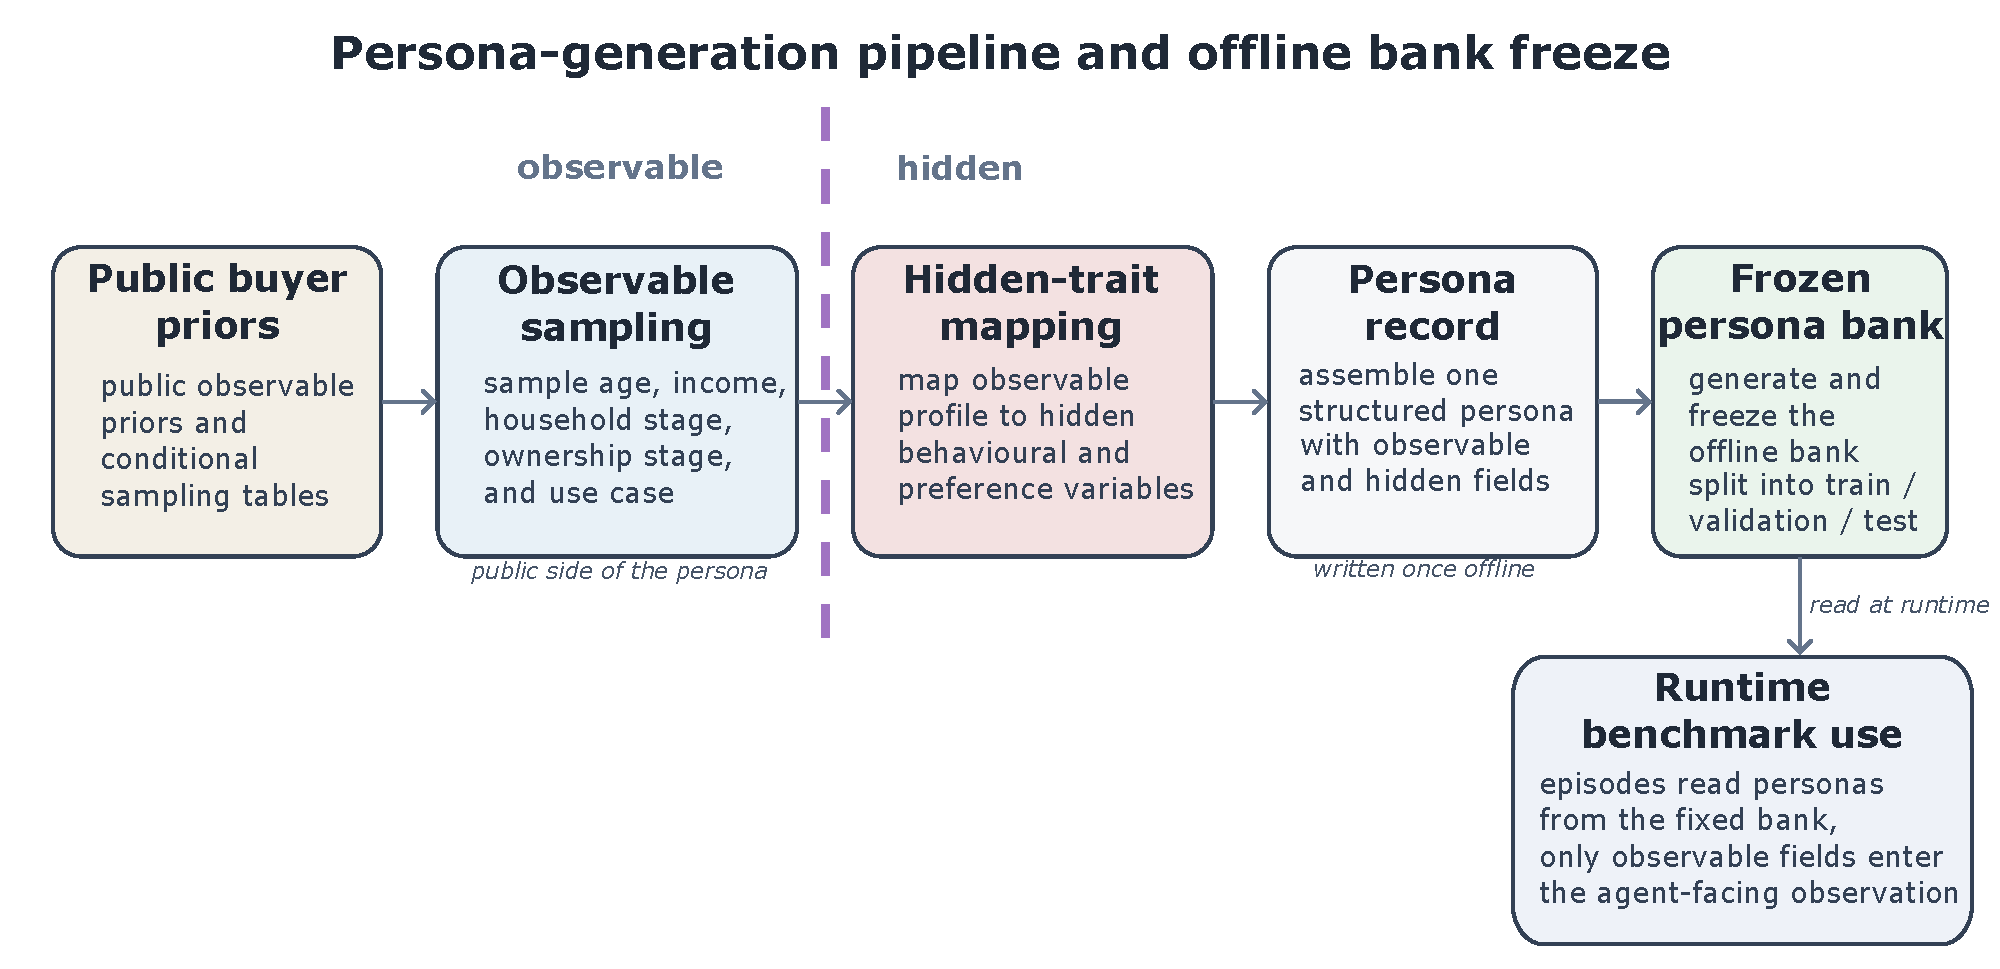
\includegraphics[width=0.85\linewidth]{ch4/ch4_persona_pipeline.pdf}
  \caption{Persona generation pipeline used by the benchmark prototype. Observable profile variables and hidden buyer traits are generated before episodes are evaluated under a fixed persona bank.}
  \label{fig:persona_pipeline}
\end{figure}

\subsection{Interaction Protocol}

The interaction protocol is shared across agents. Each policy is evaluated on the same test split and seed-controlled episode stream, so differences in outcomes are attributable to policy behavior rather than to different buyer samples. The benchmark records seller actions, buyer responses, termination reason, deal outcome, profit, and round count for each episode.

\begin{figure}[t]
  \centering
  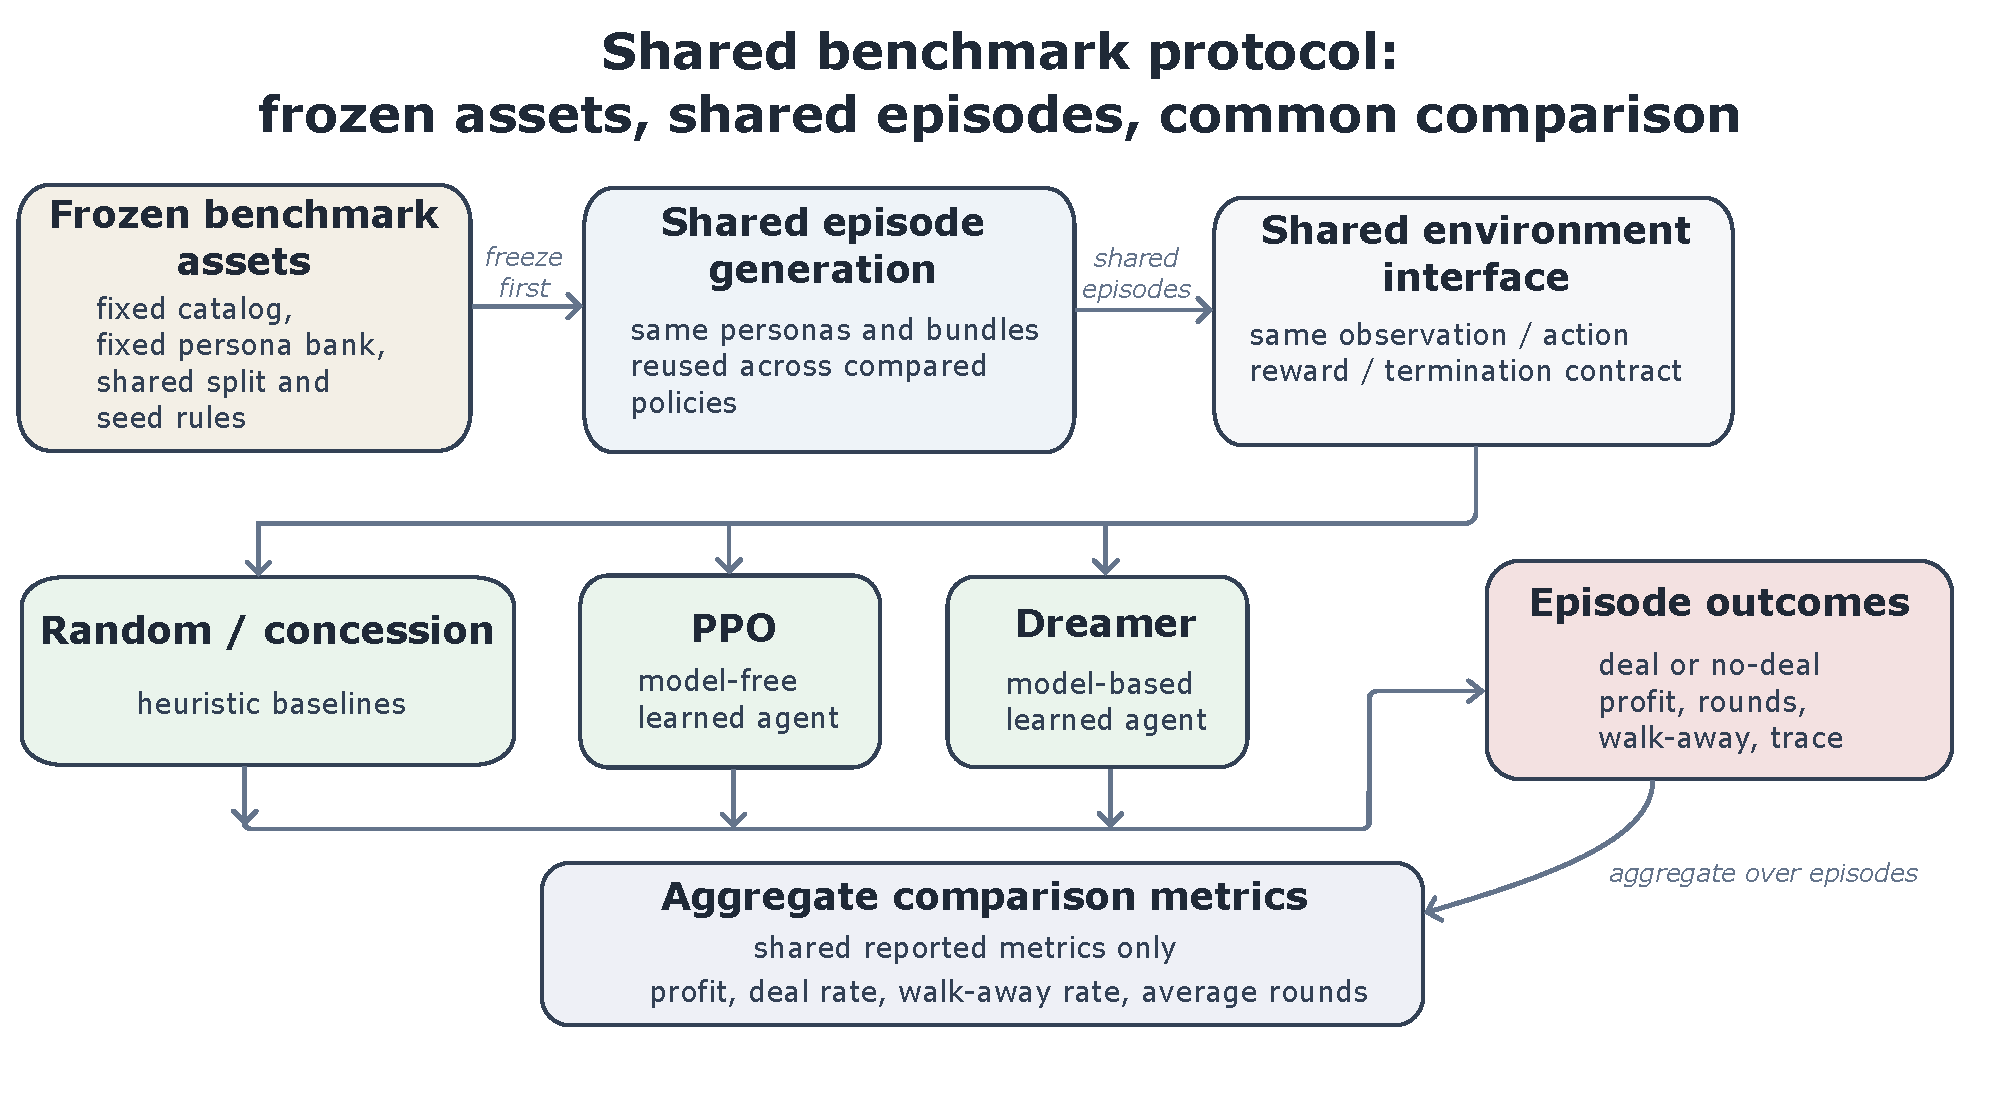
\includegraphics[width=0.85\linewidth]{ch4/ch4_shared_protocol.pdf}
  \caption{Shared benchmark protocol. All agents interact with the same environment contract and are evaluated with the same episode-level metrics.}
  \label{fig:shared_protocol}
\end{figure}

\subsection{Metrics}

The primary metric is average seller profit, because the task is seller-facing pricing. We also report deal rate, walkaway rate, and average rounds. These metrics are reported together because agreement frequency and profit are not equivalent: an agent can close many deals by pricing too softly, while a more conservative agent may preserve margin at the cost of more failed negotiations.

\section{Baseline Agents}
\label{sec:agents}

The prototype currently includes checkpoint-free heuristic baselines. Their role is not to solve the pricing problem, but to provide interpretable anchors for the benchmark before adding zero-shot LLM agents.

\paragraph{Random policy.}
The random policy samples offer prices from a fixed feasible range, occasionally accepts a buyer counter-offer, and occasionally walks away. It serves as a sanity baseline for checking whether the environment rewards meaningful pricing behavior.

\paragraph{Concession policy.}
The concession policy starts from a high-margin offer and lowers its target price as the negotiation progresses. When a buyer counter-offer is available, it partially adapts toward that counter-offer while preserving a minimum margin. This policy is intentionally simple and inspectable, making it a useful reference for future LLM baselines.

\paragraph{LLM-facing extension.}
The current report does not yet include a broad LLM-agent study. The planned extension is a natural-language observation renderer with a structured JSON action schema, so zero-shot LLM agents can participate under the same simulator contract as the heuristic policies. Prompt optimization, fine-tuning, and large-scale model leaderboards are left to future work.

\section{Experiments}
\label{sec:experiments}

The current experiments compare checkpoint-free heuristic agents under one shared benchmark protocol. All methods are evaluated on the same frozen test split and seed-controlled episode stream. The table below summarizes retained heuristic baseline results over \(5000\) test episodes.

\begin{table}[t]
  \centering
  \caption{Heuristic benchmark comparison on the test split under the shared evaluation protocol.}
  \label{tab:core_benchmark_results}
  \small
  \begin{tabular}{lrrrr}
    \toprule
    Method & Avg Profit (USD) \(\uparrow\) & Deal Rate \(\uparrow\) & Walkaway Rate \(\downarrow\) & Avg Rounds \\
    \midrule
    Random & 6058.8570 & 0.5796 & 0.4204 & 1.3208 \\
    Concession & \textbf{14725.4262} & \textbf{0.7244} & \textbf{0.2756} & \textbf{1.7196} \\
    \bottomrule
  \end{tabular}
\end{table}

These results show that the environment separates weak random pricing from a simple structured negotiation heuristic. The concession policy achieves higher seller profit and a higher deal rate than random behavior, which indicates that the benchmark rewards coherent price adaptation rather than merely ending negotiations quickly.

The current result set is intentionally compact. It establishes a runnable benchmark artifact and heuristic reference points. The next experimental step is to add zero-shot LLM baselines under the same fixed episode stream and to report invalid-output rate, API cost, and token usage alongside negotiation metrics.

\section{Limitations and Future Work}
\label{sec:limitations}

PrefBench is a benchmark prototype, and its limitations are part of the release contract.

\paragraph{Simulator-based data.}
The buyer population is semi-synthetic. Observable variables are configured from plausible population assumptions, while hidden preferences and negotiation traits are generated by hand-designed conditional rules. The benchmark should therefore be used for controlled study of personalized pricing agents, not as evidence of deployable real-world pricing performance.

\paragraph{Limited external validation.}
The current release does not include a large human-subject study or real transaction data. Future work should add human reference evaluation, expert review of buyer behavior, or small-scale preference elicitation to calibrate parts of the latent model.

\paragraph{Limited LLM evaluation.}
The current prototype is designed to support future LLM-facing evaluation, but the reported results focus on heuristic baselines. A natural next step is to add a natural-language observation renderer, a structured JSON action schema, and low-cost zero-shot LLM baselines.

\paragraph{Diagnostic extensions.}
The hidden variables in the simulator make belief probing possible: one can ask whether an agent or probe model can infer price sensitivity, patience, bargaining strength, or willingness-to-pay buckets from partial negotiation history. Robustness suites and out-of-distribution persona splits are also important future extensions.

\section{Conclusion}
\label{sec:conclusion}

This report presents PrefBench, a working benchmark prototype for personalized pricing and negotiation under hidden buyer preferences. The benchmark provides a structured product catalog, a semi-synthetic persona bank, a multi-round negotiation environment, and a shared evaluation protocol for comparing pricing agents. The current baseline results provide checkpoint-free heuristic anchors and show that structured concession behavior outperforms random pricing under the retained protocol. The current release is best understood as a reproducible artifact and starting point for future benchmark development, especially LLM-facing evaluation, belief probing, robustness testing, and human reference comparison.


\clearpage
\bibliographystyle{unsrtnat}
\bibliography{data/UG_Thesis}

\end{document}
